\documentclass{article}

\usepackage{Style_Thesis-Report}

\title{Probability}
\author{Ignacio Sada S\'{o}lomon}
\date{Winter 2020}  %Place'%' at front to activate today's date


\begin{document}
\clearpage\maketitle
\thispagestyle{empty}
\vspace{2cm}

\begin{abstract}
	Sample space, events, conditional probability, independence of events, Bayes' Theorem. Basic combinatorial probability, random variables, discrete and continuous univariate and multivariate distributions. Moment generating functions Independence of random variables. Chebyshev’s inequality,central limit theorem, weak law of large numbers (if time allows).
\end{abstract}

\newpage

\tableofcontents
\newpage
\setcounter{page}{1}
\cfoot{\thepage}

\section{Fundamentals}
\subsection{Set Theory}

	\begin{defn}
		A \textbf{set} is a collection of objects, called elements.
	\end{defn}
	\begin{exmp}
		The set of natural numbers $\N = \{ 1, 2, 3, \dots\}$, which is both infinite and countable.
	\end{exmp}
	\begin{exmp}
		The set of all McGill students.
	\end{exmp}
	\begin{defn}
		Let $X$ be a set. A \textbf{subset} is another set $A$ such that every element of $A$ is in $X$ as well:
		$$ A = \{ x: x \in X\} \quad \text{ or } \quad x \in A \implies x \in X$$
	\end{defn}
	\begin{rem}
		The empty set is denoted $\varnothing = \{\}$
	\end{rem}
	\begin{defn}
		An \textbf{intersection} between the sets A and B is defined as
		$$ A \cap B = x \in A \quad \text{and}\quad x \in B$$
	\end{defn}
	\begin{defn}
		A \textbf{union} between the sets A and B is defined as
		$$ A \cup B = x \in A \quad \text{or}\quad x \in B$$
	\end{defn}
	\begin{defn}
		Let $X$ be a universal set with a subset $A$. Then the complement of $A$ with respect to $X$ is
		$$ A^c = X \setminus A = \{ x: x \in X \quad \text{and} \quad x \notin A \}$$
	\end{defn}
	\begin{exmp}
		$\mathcal{P} (B) = \{ A: A \subseteq B \}$ (all subsets of $B$)
		
		Let $B = \{1,2,3\}$, then
		$$ \mathcal{P}(B) = \bigg\{ \underbrace{ \{\}, \{1,2,3\}}_{\text{trivial subsets}}, \underbrace{\overbrace{\{1\}, \{2\}, \{3\},}^{\text{singletons}} \overbrace{\{1,2\}, \{1,3\}, \{2,3\}}^{\text{doubles}}}_{\text{proper subsets}} \bigg\}$$
	\end{exmp}
	\begin{defn}
		Two sets $A$ and $B$ are denoted as \textbf{disjoint} whenever they share no elements, i.e. they have nothing in common:
		$$ A \cap B = \varnothing$$ 
	\end{defn}
	\begin{exmp}
		Let $\Omega = \N = \{ 0,1,2,3,4,\dots\}$ and $A \subseteq N = \{ n \in \N: n \text{ is even}\}$. Then,
		$$ A^c = \{ n \in \N : n \text{ is odd}\}$$
	\end{exmp}
\pagebreak
\subsubsection{Properties of Sets}
	\begin{multicols}{2}
		\begin{itemize}
			\item $A \cap \varnothing = \varnothing$
			\item $A \cup \varnothing = A$
			\item $A \cup B = B \cup A$
			\item $A \cap B = B \cap A$
			\item $(A\cap B)\cap C = A \cap (B \cap C)$
			\item $(A \cup B) \cup C = A \cup (B \cup C)$
			\item $(A \cap B)^c = A^c \cup B^c$
			\item $(A \cup B)^c = A^c \cap B^c$
		\end{itemize}
	\end{multicols}
	\begin{exe}
		Prove that
		\begin{enumerate}[$\quad \quad$a)]
			\item $A \cup (B \cap C) = (A \cup B) \cap (A \cup C)$
			\item $A \cap (B \cup C) = (A \cap B) \cup (A \cap C)$
		\end{enumerate}
	\end{exe}
	\begin{note}
		Consider $A \setminus B = \{ x\in A: x \notin B \}$. Then we define the \textbf{exclusive or} as
		$$ A \setminus B \cup B \setminus A = A \triangle B$$
	\end{note}
\pagebreak
\section{Probability}
	\subsection{Introduction}
	Probability is the branch of applied mathematics that deals with random events, which are non-deterministic in nature, unlike calculus for instance, which deals with deterministic events.
	\begin{exmp}
		Toss a coin. We won't know the outcome of the toss, but we do know that the outcome will be either \emph{heads} or \emph{tails}.
	\end{exmp} 
	\begin{exmp}
		Roll a die. We now have several outcomes, depending on the number of faces on the die.
	\end{exmp}
	\begin{defn}
		Given a random experiment, the set of all possible outcomes is denoted $\Omega$, and is called the \textbf{sample space}.
	\end{defn}
	\begin{exmp} $\quad$ \\
		\vspace{-0.5cm}
		\begin{itemize}
			\item The sample space for a coin toss is $\Omega = \{ H, T \}$
			\item The sample space for a rolled 6-face die is $\Omega = \{1,2,3,4,5,6\}$
			\item The sample space for a coin toss where we require heads once is $\Omega = \{ H, TH, TTH, \dots \}$
		\end{itemize}
	\end{exmp}
	\begin{defn}
		Let $\Omega$ denote the set of all possible outcomes of a random experiment.
		\begin{enumerate}[$\quad\,\,${2.2}.1.]
			\item An \textbf{elementary event} is a subset of $\Omega$ with a singular element (i.e. one single outcome) and is also an element of $\mathcal{P}(\Omega)$.
			\item A \textbf{compound event} is any subset of $\Omega$ (including the elementary events).
			\item An \textbf{event} is any element of $\Omega$.
			\item $\varnothing$ denotes \textbf{impossible events}.
			\item A \textbf{complimentary event} given an event $A$ is denoted $A^c$.
			\item Given 2 events $A$ and $B$, where $A \cap B = \varnothing$, we denote them as \textbf{disjoint events}.
		\end{enumerate}
	\end{defn}
	\begin{defn}
		Let $\Omega$ be the sample space attached to a random experiment. A \textbf{probability} is a function $P$ such that
		$$ P: \mathcal{P}(\Omega) \to [0,1]$$
	\end{defn}
	Note that $P(\Omega)=1$. Given a sequence $A_1, \dots, A_n, \dots$, of pairwise disjoint events ($A_i \cap A_j = \varnothing \quad \forall i \neq j$), we have that 
	$$ P \left(  \bigcup_{i =1} A_i\right) = \sum_{i =1} P (A_i)$$
	\begin{rem}
		In general, if $\Omega$ is countable, then it is enough to define $P$ on the elementary event, as every other event can be written as a union.
	\end{rem}
	\begin{exmp}
		Toss a coin such that $\Omega = \{ H, T \}$. A probability on $\Omega$ is completely given by $p \in [0,1]$, and the assignment of $P(\{H\}) = p$, and $P(\{T\}) = 1-p$.
	\end{exmp}
	\begin{rem}
		If $p=1/2$ in the previous example, then $P(\{H\}) = P(\{T\}) = 1/2$, implying that \emph{the coin is fair/balanced}.
	\end{rem}
	\begin{exmp}
		Throw a die such that $\Omega = \{ \omega_1, \omega_2, \omega_3, \omega_4, \omega_5, \omega_6 \}$. A probability on $\Omega$ is given by 6 non-negative integers $p_i$ where $i=1,2,3,4,5,6$, such that
		$$ p_i = P(\{w_i\}) \geq 0$$
		And so
		$$ \sum_{i=1}^6 p_i = 1$$
		Therefore, if we consider the die to be fair, we have $p_i = 1/6 \quad \forall i \in \{ 1,2,3,4,5,6 \}$. \\ Let $A = \{ \omega_1, \omega_3\}$ Then
		\begin{align*}
		 A &= \{ \omega_1\} \cup \{ \omega_3 \} \implies P(A) \\ 
		 &= P(\{ \omega_1 \}) + P(\{ \omega_3 \}) \\
		 &= 1/6 + 1/6 \\
		 &= 1/3
		\end{align*} 
	\end{exmp}
	\begin{exe}
		Consider a die such that the probability $P(\{\omega_i\})$ is proportional to $k$ such that
		$$ P \big( \{\omega_i\} \big) = ck$$
		Therefore:
		\begin{align*}
			1 &= \sum_{k=1}^6 P(\{\omega_k\}) \\
			&= \sum_{k=1}^6 ck \\
			&= c\sum_{k=1}^6 k \\
			&= c\frac{n(n+1)}{2}\bigg|_{n=6} 
				\intertext{}
			&= c \frac{6 \times 7}{2} \\
			&= 21c\\
			\therefore c &= \frac{1}{21}
		\end{align*}
		
		What would be the probability of an even number?\\
		Let $A = \{ \omega_2, \omega_4, \omega_6 \}$, and so
		\begin{align*}
			P(A) &= P(\{\omega_2\}) + P(\{\omega_4\}) + P(\{\omega_6\})  \\
			&= \frac{2+4+6}{21} \\
			&= \frac{12}{21}
		\end{align*}
		
		What would be the probability of an odd number?\\
		Simple:
		\begin{align*}
			P(B) &= 1- P(A) \\
			&= \frac{9}{21}
		\end{align*}
	\end{exe}
	\begin{exmp}
		Toss a coin until heads appears. We then have:
		$$ \Omega = \{ \omega_1 = H, \omega_2 = TH, \omega_3 = TTH, \dots, \omega_n = \underbrace{TTT}_{n-1}H, \dots \}$$
		$$ \therefore P \big( \{ \omega_n \} \big) = c \left( \frac{1}{3}\right)^n$$
		We now let $1 = c \left( \sum_{n=1}^\infty \left( \frac13\right)^n \right)$ such that
		\begin{align*}
			c &= \frac{1}{\sum_{n=1}^\infty \left( \frac13 \right)^n} \\
			&= \frac{1}{\frac{1}{3} \left( \frac{1}{1-1/3} \right)} \\
			&= \frac{1}{\frac{1}{3} \left( \frac{3}{2} \right)} \\
			&= \frac{1}{\frac12}\\
			&= 2
		\end{align*}
\pagebreak

		Thus, $P \big( \{ \omega_n \} \big) = 2 \left(\frac{1}{3}\right)^n \implies H$ appears in an even number of trials. Then, what is $P(A)$? Recall that \\ $A = \{ \omega_1, \omega_2, \dots, \omega_n, \dots\} $ so \\
		\vspace{-1cm}
		\begin{align*}
			P(A) &= \sum_{n=1}^\infty P \left( \{ \omega_n \} \right) \\
			&= \sum_{n=1}^\infty 2 \left( \frac13 \right)^{2n} \\
			&= 2 \sum_{n=1}^\infty \left( \frac{1}{3^2} \right)^{2n} \\
			&= 2 \cdot \frac19 \left( \frac{1}{1-\frac{1}{9}}\right) \\
			&= \frac14
		\end{align*}
	\end{exmp}
	\begin{thm}
		Let $A, B$ be subsets of a set $\Omega$. The probability function $P: \Omega \to [0,1]$ has the following properties:
		\begin{enumerate}[$\quad\quad$1)]
			\item $P(\varnothing) = 0$ 
			\item $P(A^c) = 1 - P(A)$
			\item $P(A \cup B) =  P(A) + P(B) - P(A \cap B)$
		\end{enumerate}
	\end{thm}
	\begin{proof}
		\begin{enumerate}[$\quad\quad$1)]
			\item 
			\begin{align*}
				\Omega = \Omega \cup \varnothing &\iff \Omega \cap \varnothing = \varnothing \\
				&\iff P(\Omega) = P(\Omega \cup \varnothing)\\
				&\iff P(\Omega) + P(\Omega) \\
				&\iff 1= 1+ P(\varnothing) \\
				&\iff P(\varnothing) = 0
			\end{align*}
			\item 
			\begin{align*}
				\Omega = A \cup A^c &\iff A \cap A^c = \varnothing \\
				&\iff 1 = P(\Omega) = P(A) + P(A^c)\\
				&\iff P(A^c) = 1 - P(A)
			\end{align*}
			\item
			\begin{align*}
				A \cup B = (A \setminus B) \cup B &\iff (A \setminus B) \cap B = \varnothing \implies P(A \cup B) = P(A \setminus B) + P(B)\\
				\therefore A = (A\setminus B) \cup (A \cap B) &\iff (A \setminus B) \cap (A \cap B) = \varnothing \implies P(A) = P(A \setminus B) + P(A \cap B) \\
				&\iff P(A \setminus B) = P(A) - P(A \cap B) \\
				\therefore P(A \cup B) &= P(A) + P(B) - P(A \cap B)
			\end{align*}
		\end{enumerate}
	\end{proof}
	\begin{exe}
		Show that $P(A \cup B \cup C) = P(A) + P(B) + P(C) - P(A \cap B) - P(A \cap C) -  P(B \cap C) + P(A \cap B \cap C)$
	\end{exe}
	\begin{defn}
		Let $\Omega_1, \Omega_2$  be two finite sample spaces.
		\begin{enumerate}[$\quad\quad$1)]
			\item $\Omega_1 \times \Omega_2 = \{ (\omega_1, \omega_2): \,\,  \omega_1 \in \Omega_1, \,\,  \omega_2 \in \Omega_2 \}$
			\item $|\Omega_1 \times \Omega_2| = |\Omega_1| \cdot |\Omega_2|$
		\end{enumerate}
	\end{defn}
	\begin{exmp}
		Roll a die twice. What is the probability that the sum of the number obtained is 7? We will define the set of events where the sum of both rolls is 7 as $A$:
		\begin{align*}
			\Omega = \Omega_1 \times \Omega_2 \implies |\Omega| = |\Omega_1| \cdot |\Omega_2| = 36 \\
			\Omega_1 = \Omega_2 = \{ \omega_1, \omega_2, \omega_3, \omega_4, \omega_5, \omega_6 \}
		\end{align*}
		Thus,
		\begin{align*}
			A = \{ (\omega_1, \omega_6), (\omega_2, \omega_5), &(\omega_3, \omega_4), (\omega_4, \omega_3), (\omega_5, \omega_2), (\omega_6, \omega_1)  \} \\
			\therefore P(A) &= \frac{|A|}{|\Omega|} = \frac{6}{36} = \frac16
		\end{align*}
	\end{exmp}
	\begin{exe}
		Find the probability such that the sum of the number obtained in both rolls is even. 
		\\
		(\emph{Ans: 1/2})
	\end{exe}
	\begin{defn}
		A \textbf{permutation} of $r$ elements chosen from $n$ elements is equivalent to throwing successively without replacement $r$ elements from a urn which contains $n$ elements. The total number of combinations for a permutation is
		$$ C_r^n = \binom{n}{r} = \frac{P_r^n}{r!} = \frac{n!}{r! (n-r)!} $$
	\end{defn}
	Note that:
	$$ P_r^n = n(n-1)(n-2)\dots (n-r+1) = \frac{n!}{(n-r)!}$$
	is the number of possible combinations.
	\begin{exmp}
		A urn contains 4 balls; 1 green ball, 1 blue ball, 1 red ball, and 1 yellow ball. Draw successively without replacement 3 balls from the urn.
	\end{exmp}
	\begin{exmp}
		A hand is a subset of 5 cards from a deck of 52 cards.
		$$ C_r^n = C_5^{52} = \frac{52!}{5! (47!)} = \frac{48 \times 49 \times 50 \times 51 \times 52}{1 \times 2 \times 3 \times 4 \times 5}$$
		What is the probability that a selected (or random) hand will contain at least one Jack?
		Let $A = $``At least 1 Jack" such that  $A^c =$ ``No jack". Then,
		\begin{align*}
			P(A^c) &= \frac{C^{48}_5}{C^{52}_5} &P(A) = 1-P(A^c)
		\end{align*}
		If we let $A_i = $``At least $i$ Jacks" for $i=1,2,3,4$, then
		\begin{align*}
			P(A) &= P\left( \bigcup_{i=1}^4 A_i \right)  \\
			&= \sum_{i=1}^4 P(A_i) &P(A_i) = \frac{C_i^4 \times C_{5-i}^{48}}{C_{5}^{52}}
		\end{align*}
		\begin{rem}
			$C_r^n$ is the number of subsets with $r$ elements of a set $S$ which has $n$ elements.
		\end{rem}
		Consider this alternative solution:
		\begin{align*}
			P(A) &= 1 - \overbrace{P(A^c)}^{\text{No jack}} \\
			\therefore P(A^c) &= \frac{C_{5}^{48}}{C_5^{52}} \implies P(A) = 1- \frac{C_{5}^{48}}{C_5^{52}} 
		\end{align*}
	\end{exmp}
	\begin{exe}
		The letters of the word ``ANANAS" are written on 6 marbles. Select 3 marbles successively, without replacement, from the initial 6 marbles to form a 3 letter word.
	\end{exe}
\hfill
	\begin{thm}
		\textbf{The Binomial Theorem:}
		$$ (a+b)^n = \sum_{k=0}^n C_k^n a^{k}b^{n-k} $$
	\end{thm}
	\begin{exmp}
		$(a+b)^4 = b^4 + 4ab^3 + 6a^2b^2 + 4a^3 b + a^4$
	\end{exmp}
	\begin{exmp}
		Find the coefficient of $x^7$ in the expansion of $(2+3x^2)^6$ \\
		(\emph{Ans: $C_{4}^5 3^4 2^3$})
	\end{exmp}
\pagebreak

	We can apply this concept to find the \emph{power set of a fine set}. Let $\Omega$ be a finite set. $\mathcal{P}(\Omega)$ is the power set of $\Omega$. If $|\Omega| = n$, then $|\mathcal{P}(\Omega)|$ is
	\begin{align*}
		|\mathcal{P}(\Omega)| &= C_0^n + C_1^n + C_2^n + \dots + C_k^n + \dots + C_n^n \\
		&= \sum_{k=0}^n C_k^n \\
		&= \sum_{k=0}^n (1)^k (1)^{n-k} C_k^n \\
		&= (1+1)^n \\
		&\boxed{= 2^n}
 	\end{align*}
	
	\begin{exmp}
		\begin{align*}
			(a+b)^4 &= \sum_{k=0}^4 C_k^4 a^k b^{4-k} \\
			&= b^4 + 4ab^3 + 6a^2 b^2 + 4a^3 b + a^4
		\end{align*}
	\end{exmp}
\hfill
\subsection{Conditional Probability}
	Consider rolling a fair die. The probability that we obtain 2 as a result is $\frac{1}{6}$. However, the probability of obtaining 2 from only even numbers is $\frac{1}{3}$.
	
	\begin{defn}
		Let $\Omega$ be a parent set of events, and let us consider subsets of events $A \subset \Omega$ and $B \subset \Omega$.  Then, the \textbf{conditional probability} of $A$ given $B$ is
		$$ P(A \mid B ) = \frac{P (A \cap B)}{P(B)}$$
	\end{defn}
	\begin{center}
		\begin{tikzpicture}
		\draw \firstcircle node[below]{$A$};
		\draw \secondcircle node[below]{$B$};
		\draw (-2cm, -2cm) -- (4cm, -2cm) -- (4cm, 2cm) -- (-2cm, 2cm) -- (-2cm, -2cm) node[above=4mm, right=2mm]{$\Omega$};
		\begin{scope}
			\clip \firstcircle;
			\fill[grey!40] \secondcircle;
		\end{scope}
		\end{tikzpicture}
	\end{center}
	\begin{rem}
		The map $A \mapsto P(A \mid B)$ is a probability on $\mathcal{P}(\Omega)$.
	\end{rem}
\pagebreak
	\begin{exmp}
		Throw a fair die. We define the following events:
		\begin{multicols}{3}
			\begin{itemize}
				\item $A= $ result is even.
				\item $B= $ either 1, 2, or 5
				\item $C= $ either 1 or 2
			\end{itemize}
		\end{multicols}
		Thus:
		\begin{align*}
		P(A)  = \frac12 && P(B) = \frac12 && P(C) = \frac13 &&  \\
		 P(A \cap C) = \frac16 && P(B \cap C) = \frac13 && P (A \cap B) = \frac16 && \\
		\intertext{Hence:}
		P(A \mid B) = \frac{P(A \cap B)}{P(B)} = \frac13 && P(A \mid C) = \frac{P(A \cap C)}{P(C)} = \frac12  &&P(B\mid A) = \frac{P(A \cap B)}{P(A)} = \frac13 && \\
		 P(C \mid A) = \frac{P(A \cap C)}{P(A)} = \frac13 && P(B \mid C) = \frac{P(B \cap C)}{P(C)} = 1 && P(C\mid B) = \frac{P(B \cap C)}{P(B)} = \frac23 &&
		\end{align*}
	\end{exmp}

	\begin{defn}
		Two events $A$ and $B$ are said to be \textbf{independent} if at least one of the following statements is true:
			\begin{multicols}{3}
			\begin{itemize}
				\item $P(B \mid A) = P(B)$ 
				\item $P(A \mid B) =P(A)$
				\item $P(A \cap B) = P(A ) P(B)$
			\end{itemize}
		\end{multicols}
	\end{defn}
	\begin{exmp}
		In Example 2.13:    
		\begin{itemize}
			\item$A$ and $B$ are not independent $\left(P(A \cap B) = \frac16, \quad P(A)P(B) = \frac14\right)$
			\item $A$ and $C$ are independent $\left(P(A \cap C) = \frac16, \quad P(A)P(C) = \frac16\right)$
			\item $B$ and $C$ are not independent $\left(P(B\cap C) = \frac13, \quad P(B)P(C) = \frac16\right)$
		\end{itemize}
	\end{exmp}
	\begin{exmp}
		Toss a coin (which is such that $P(H) = p \in (0,1)$)twice. What is the probability that we will obtain $T$ twice? 
		$$ P (\underbrace{\{ T\} \times \{T\} }_{TT} )$$ 
		By design, the outcome obtained on the first toss is \emph{independent from the outcome obtained in the second toss:}
		\begin{align*}
			P(TT) &= P \big( \{T\} \big) \times  P \big( \{T\} \big) \\
			&= (1-p)^2
		\end{align*}
	\end{exmp}
	\begin{exmp}
		Toss a coin such that $P \big(  \{H\} \big) = p \in (0,1)$ until $H$ appears. 
		\begin{sol}
			We have:
			$$ \Omega = \{ H, TH, TTH, TTTH, \,\, \dots\, \, , \underbrace{T\dots T}_{n-1}H \}$$
			\begin{align*}
			\therefore P(\omega_n) &= \big( P(T) \big)^{n-1} \times \big( P(H) \big) \\
			&= (1-p)^{n-1} \times (p)
			\intertext{We now recall infinite series expansion to evaluate $P(\omega_n)$:}
			\sum_{n=1}^\infty (1-p)^{n-1} (p) &= p \sum_{n=1}^\infty (1-o)^{n-1} \\
			&= p \sum_{n=0}^\infty (1-p)^n \\
			&= p \left( \frac{1}{1-(1-p)} \right) \\
			&= 1
			\end{align*}
		\end{sol}
 	\end{exmp}
 \begin{thm}
 	If $A$ and $B$ are independent ($A \perp B$), then so are $A^C$ and $B^C$. Consequently:
 	\begin{align*}
 		A^C \perp B && B^C \perp A
 	\end{align*}
 \end{thm}
	\begin{proof}
		\begin{align*}
			P(A^C \cap B ) &= P (B \setminus A) \\
			&= P(B) - P(A \cap B) \\
			&= P(B) -P(A)P(B) \\
			&= P(B) - (1- P(A)) \\
			&= P(B) P(A^C)
		\end{align*}
		$B^C$ and $A$ are similarly shown to be independent.
	\end{proof}
	\hfill
	\begin{exmp}
		Let $P(A) = 0.7$, $P(B)=0.8$, $A$ and $B$ are independent ($A \perp B$). Find $P(A^C \cap B^C)$.
	\pagebreak
		\begin{sol}
			$ $
			\begin{align*}
				P(A^C\cap B^C) &= P(A^C)P(B^C)\\
				&= (0.3)(0.2)\\
				&\boxed{= 0.06}
			\end{align*}
		\end{sol}
	\end{exmp}
	\begin{exmp}
		Let $P(A) = 0.7$, $P(B)=0.8$, $A$ and $B$ are independent ($A\perp B$). Find $P(A \cup B)$.
		\begin{sol}
			\begin{align*}
				(A \cup B)^C &= A^C \cap B^C \\
				&= P(A) + P(B) - P(A \cap B) \\
				&= P(A) + P(B) - P(A)P(B)\\
				&= 0.7 + 0.8 - 0.56 \\
				&\boxed{=0.94}
			\end{align*}
		\end{sol}
	\end{exmp}
 	\begin{exe}
 		A die is such that $P\big( \{ \omega_2 \} \big) = p$, $P\big( \{\omega_4\} \big) = q$, and $p+q \in (0, 1)$. Roll the die until 2 or 4 appears. What is the probability that 2 appears first?\\
 		(\emph{Ans: $\frac{p}{p+q}$} )
 	\end{exe}
\subsection{Baye's Rule}
	\begin{exmp}
		On a given exam, we are given the following distribution:
		\begin{table}[h]
			\begin{tabular}{c|c|c|c}
				& Success (S) & Failure (Fl) & Total \\ \hline
				Male (M)   & 0.3         & 0.1         & 0.4   \\ \hline
				Female (Fm) & 0.4         & 0.2         & 0.6   \\ \hline
				Total      & 0.7         & 0.3         & 1    
			\end{tabular}
		\end{table}
		Here,
		\begin{center}
			\begin{multicols}{2} 
				\begin{itemize}
					\item $P(M) = 0.4$
					\item $P(Fm) = 0.6$
					\item $P(S \mid M) = \frac34$
					\item $P(S \cap M)=0.3$
					\item $P(S \cap Fm)=0.4$
					\item $P(S \mid Fm) = \frac23$
				\end{itemize}
			\end{multicols}
		\end{center}
		Thus, 
		\begin{align*}
			P(S) &= P(M \cap S) + P(Fm\cap S)  \\
			&= P (S \mid M) P(M) + P (S \mid Fm) P(Fm) \\
			&= \left( \frac34 \times \frac{4}{10} \right) + \left( \frac23 \times \frac{6}{10} \right)\\
			&\boxed{= \frac{7}{10}} 
		\end{align*}
	\end{exmp}
	\begin{defn}
		Let $\Omega$ be a sample space. A \textbf{finite partition } of $\Omega$ is given by events $A_1, A_2, A_3, \,\, \dots, A_n$, which are pairwise disjoint, and also 
		$$ \bigcup_{n \in \N^*} A_n= \Omega $$
	\end{defn}
	\begin{figure}[h]
		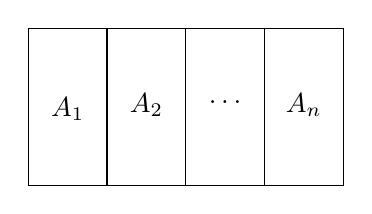
\begin{tikzpicture}
			\draw (0,0) -- (4, 0) -- (4, 2) -- (0,2) -- (0,0) node[right= 5mm, above=7mm]{$A_1$};
			\draw (1, 0) -- (1, 2) node[right= 5mm, below=7mm]{$A_2$} ;
			\draw (2, 0) -- (2, 2) node[right= 5mm, below=8mm]{$\dots$} ;
			\draw (3, 0) -- (3, 2) node[right= 5mm, below=7mm]{$A_n$};
		\end{tikzpicture}
	\end{figure}
	
	\begin{thm} \textbf{Baye's Theorem}\\
		Given a partition $A_1, A_2, \,\dots, A_n$ of $\Omega$, suppose that $P(A_1)$, $P(A_2)$, $\dots$, $P(A_n)$ are known. Suppose that for an event $B$, the following are known: $P(B \mid A_1), P(B \mid A_2), \dots, P(B \mid A_n)$. Thus:
		\begin{enumerate}
			\item $\quad$ 
			\begin{center}
				$P(B) = \sum_{i= 1}^n P(B \mid A_i) P(A_i) $
			\end{center}
			
			\item Let $k \in \{1, 2, \dots, n\}$ be fixed. Then: $$ P(A_k \mid B ) = \frac{P (B \mid A_k) P(A_k)}{\sum_{i=1}^n P(B\mid A_i) P(A_i)}$$
		\end{enumerate}
	\end{thm}
	\begin{proof}
		Let $B = \Omega$, then:
		\vspace{-1cm}
		\begin{align*}
			B &= B \cap \left( \cup_{n \in \N^*} A_n \right) \\
			&= \cup_{n \in \N^*} \left( B \cap A_n \right) \\
			\therefore P(B) &= \sum_{k=1}^n P(B \cap A_k) \\
			\therefore P(A_i \mid B) &= \frac{P(B \cap A_i)}{P(B)} \\
			&= \frac{P(B \mid A_i) P(A_i)}{P(B)}
		\end{align*}
	\end{proof}
	\begin{exmp}
		We have 2 urns. Urn 1 has 3 red balls and 2 blue balls, and urn 2 has 5 red balls and 6 blue balls. We now select a ball from urn 1, place it in urn 2, and select a ball from urn 2. What is the probability that said ball is red?
		\begin{sol}
			Let $A$ be the event where the ball from urn 2 is red, and $B$ where the ball from urn 1 is blue. By Baye's Theorem,
			\begin{enumerate}
				\item$ P(A) = \frac{2}{5} \cdot \frac{5}{12} + \frac{1}{2}\cdot \frac{3}{9} = \frac{7}{15}$
				\item $P(B \mid A) = \frac{5}{12} $
			\end{enumerate}
		\end{sol}
	\end{exmp}
	\begin{exmp}
		On a weather forecast model we have that:
		\begin{enumerate}[$\quad\quad$a)]
			\item If today is rainy, then tomorrow is rainy with a probability of 0.6.
			\item If today is sunny, then tomorrow is sunny with a probability of 0.7.
		\end{enumerate}
		Suppose Monday is rainy. What is the probability that Wednesday is rainy?
		\begin{sol}
			Consider the following tree structure representing the probabilities of the forecast model:
			\begin{figure}[h]
				\begin{tikzpicture}
					[sibling distance = 4cm]
					\node [root] {Rainy}
						child { 
							node [env] {Rainy} 
								[sibling distance = 2cm]
								child {
									node [env] {Rainy}
									edge from parent node [above=2mm, left] {0.6}
								}
								child {
									node [env] {Sunny}
									edge from parent node [above=2mm, right] {0.4}
								}
							edge from parent node [above=2mm, left] {0.6}
						}
						child { 
							node [env] {Sunny} 
								[sibling distance = 2cm]
								child {
									node [env] {Rainy}
									edge from parent node [above=2mm, left] {0.3}
								}
								child {
									node [env] {Sunny}
									edge from parent node [above=2mm, right] {0.7}
								}
							edge from parent node [above=2mm, right] {0.4}
						};
				\end{tikzpicture}
			\end{figure}
		
			\noindent
			Let $B = $``Wednesday is rainy",  $A_1 = $ ``Tuesday is rainy", and $A_2=$ ``Tuesday is sunny." Then,
			\begin{align*}
				P(A_1) = 0.6 &\implies P(B \mid A_1) = 0.6 \\
				P(A_2) = 0.4 &\implies P(B \mid A_2) = 0.3\\
				\therefore P(B) &= P(B \mid A_1) P(A_1) + P(B \mid A_2) P(A_2) \\
				&= (0.6)(0.6) + (0.3)(0.4) \\
				&\boxed{= 0.48}
			\end{align*}
		\end{sol}
	\end{exmp}

\subsection{Multinomial Coefficients}
	We begin by recalling that \emph{binomial coefficients} are such that a combination with $C_k^n$ is clearly defined
	
	\begin{figure}[h]
		\begin{subfigure}{0.46\textwidth}
			\begin{center}
				\begin{tikzpicture}
					[sibling distance = 3cm]
					\node [root] {$n$}  
						child{
							node [env] {$k$}
							edge from parent node [above, left=2mm]{$S_1$}
						}
						child{
							node [env] {$k-1$}
							edge from parent node [above, right=2mm]{$S_2$}
						}
					;
					\draw node [above=4mm, right=2mm]{$S$};
				\end{tikzpicture}
			\end{center}
			\caption*{Partition of a set into two subsets.}
		\end{subfigure}
		\hfill
		\begin{subfigure}{0.46\textwidth}
			\begin{center}
				\begin{tikzpicture}
				[sibling distance = 3cm]
				\node [root] {$n$}  
				child{
					node [env] {$n_1$}
					edge from parent node [above, left=4mm]{$S_1$}
				}
				child{
					node [env] {$n_2$}
					edge from parent node [above, right=1mm]{$S_2$}
				}
				child{
					node [env] {$n_3$}
					edge from parent node [above, right=4mm]{$S_3$}
				}
				;
				\draw node [above=4mm, right=2mm]{$S$};
				\end{tikzpicture}
			\end{center}
			\caption*{Partition of a set into three subsets.}
		\end{subfigure}
	\end{figure}
	We consider the above cases to generalize by induction. In the case where we have 3 partitions, we have that  $n=n_1 = n_2 = n_3$, and so the total number of partitions is
	\begin{align*}
		C_{n_1}^n &= C_{n_3}^{n- n_1} \\
		&= \frac{n!}{(n-n_3)! n!} \\
		&= \frac{n!}{n_2 ! (n-n_1 -n_3)!} \\
		&= \frac{n!}{n_1 ! n_2 ! n_3 !}
	\end{align*}
	\begin{figure}[h]
		\begin{tikzpicture}
		[sibling distance = 3cm]
		\node [root] {$n$}  
		child{
			node [env] {$n_1$}
			edge from parent node [above, left=4mm]{$S_1$}
		}
		child{
			node [env] {$n_2$}
			edge from parent node [above, right=1mm]{$S_2$}
		} 
		child{ 
			node [env] {$n_k$}
			edge from parent node [above, right=4mm]{$S_k$}
		}
		;
		\draw node [above=4mm, right=2mm]{$S$}
		node[below=1.5cm, right=1.2cm]{$\dots$};
		\end{tikzpicture}
	\end{figure}

	Now suppose that we partition a set $S$ with $n$ elements into subsets $S_1, S_2, \dots, S_k$ with respective $n_1, n_2, \dots, n_k$ elements ($\sum_i n_i = n$), so the total number of partitions is given by 
	$$
		\boxed{
		\label{eq:partno}
		\binom{n}{n, n_1, \dots, n_k} = \frac{n}{n_1 ! n_2 ! \dots n_k !}
		}
	$$
	\begin{exmp}
		10 employees are split in $k=3$ ways for $3$ different tasks. There are 3 people assigned to task 1, 2 people assigned to task 2, and 5 people assigned to task 3. Suppose that the assignment is done randomly. What is the probability that Peter and John do not belong to the same team?
	\end{exmp}
	\begin{sol}
		Recall that 
		$$ C_{n_1}^n = C_{n_{2}}^{n-n_1} = C_{n_3}^{n-n_1 - n_2}$$
		Hence:
		\begin{align*}
			C_{n_1}^n &= \frac{n!}{n_1 ! \cancel{(n-n_1)!}} \cdot \frac{\cancel{(n-n_1)!}}{n_2 ! \cancel{(n-n_1 - n_2)!}} \cdot \frac{\cancel{(n-n_1 -n_2)!}}{n_3!} \\
			&= \frac{n!}{n_1 ! n_2 ! n_3 !} \\
			&= \binom{n}{n_1, n_2, n_3}
		\end{align*}
	Generally, if there are $k$ tasks and $n$ employees, with $n_1$ employees going to task $i$, then:
	$$ \sum_{i=1}^k n_i = n$$ \noindent We thus consider the cases where both Peter and John are on the same team:
	\begin{figure}[h]
		\begin{subfigure}{0.3\textwidth}
			\begin{center}
				$A_1^C$ \\ $\quad$
				
				\begin{tikzpicture}
				[sibling distance = 2cm]
				\node [root] {8}  
				child{
					node [env] {1}
				}
				child{
					node [env] {2}
				} 
				child{ 
					node [env] {5}
				}
				;
				\end{tikzpicture}
			\end{center}
		\end{subfigure}
		\hfill
		\begin{subfigure}{0.3\textwidth}
			\begin{center}
				$A_2^C$ \\ $\quad$
				
				\begin{tikzpicture}
				[sibling distance = 2cm]
				\node [root] {8}  
				child{
					node [env] {3}
				}
				child{
					node [env] {0}
				} 
				child{ 
					node [env] {5}
				}
				;
				\end{tikzpicture}
			\end{center}
		\end{subfigure}
		\hfill
		\begin{subfigure}{0.3\textwidth}
			\begin{center}
				$A_3^C$ \\ $\quad$ 
				
				\begin{tikzpicture}
				[sibling distance = 2cm]
				\node [root] {8}  
				child{
					node [env] {3}
				}
				child{
					node [env] {2}
				} 
				child{ 
					node [env] {3}
				}
				;
				\end{tikzpicture}
			\end{center}
		\end{subfigure}
	\end{figure}

\noindent
	Hence, $$P(A^C) = \frac{A_1^C + A_2^C + A_3^C}{\left( \frac{10!}{3! 2! 5!} \right)} $$ $$ \therefore P(A) = 1 - P(A^C) = 1 - \frac{A_1^C + A_2^C + A_3^C}{\left( \frac{10!}{3! 2! 5!} \right)}$$
	\end{sol}

	\begin{thm} \textbf{Multinomial Theorem}
		$$ (a_1 + a_2 + \dots + a_k)^n = \sum_{n_1 + n_2 + \dots + n_k = n} \binom{n}{n_1, n_2, \dots, n_k} \prod_{i=1}^k a_i^{n_i}$$
		where $ \binom{n}{n_1, n_2, \dots, n_k} = \frac{n!}{n_1 ! n_2 ! \dots n_k !}$
	\end{thm}
	\begin{exe}
		Consider $(1+k + 2k^5)^7$. Find the coefficient of $k^5$.
	\end{exe}
	\begin{exmp}
		$$ (a+b+c)^3 \implies \begin{array}{ccc}
		\boxed{(3,0,0)}& (1,2,0)&\boxed{ (0,2,1)} \\
		(2,1,0) & (1,0,2) &(0,0,3) \\
		(2,0,1) & (1,1,1) & (0,3,0)
		\end{array}$$
	\end{exmp}
\pagebreak
\section{Discrete Random Variables}
	We let $\Omega$ be a sample space. We assign a number to each probable element such that the sum of all elements is one, so for $k$ elements with corresponding probabilities $p_i$ for $i=1,2,\dots, k$, we have 
	$$ \sum_{i = 0}^k p_i = 1$$
	\begin{defn}
		A \textbf{random variable} $(r, \sigma)$ is a function $X: \Sigma \to \R$ such that:
		$$ \forall \omega \in \Omega: \quad X(\omega) \in \R$$
	\end{defn}	
	\begin{exmp}
		Flip a coin, $\Omega = \{ T, H\}$. Define $X(T) = -5$, $X(H)=10$. 
	\end{exmp}
	\begin{exmp}
		Toss a die and add the numbers obtained. We have:
		$$ \Omega = \left\{ (\omega_i, \omega_j):  
		\begin{array}{c}
			i = 1,2,3,4,5,6\\
			j=1,2,3,4,5,6
		\end{array}
		\right\}$$
		$$ \therefore X: \Omega \to \R \implies X(\omega_1, \omega_2) = i +j$$
	\end{exmp}
	\begin{defn}
		A \textbf{discrete random variable} is a random variable $X: \Omega \to \R$ that is said to be discrete if its \emph{range} $X(\Omega)$ is countable. Note that it can be either finite or infinite.
		\begin{figure}[h]
			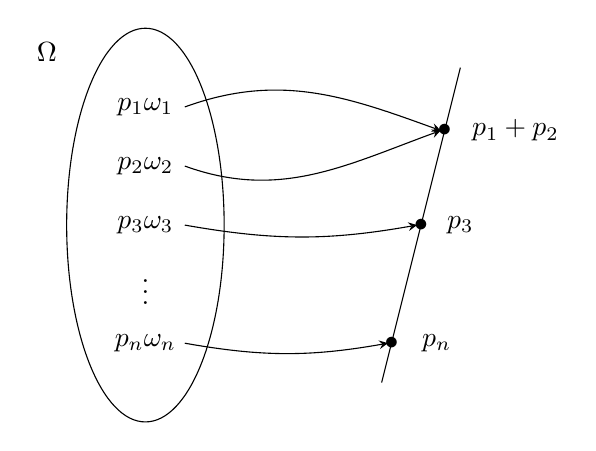
\begin{tikzpicture} 
				% Omega Ellipse
				\draw (0,0) ellipse (1cm and 2.5cm) 
					node[above=2.2cm, left=1cm]{$\Omega$}
					(0,1.5) node{$p_1 \omega_1$} 
					(0,0.75) node{$p_2 \omega_2$}  
					(0,0) node{$p_3 \omega_3$}  
					(0, -0.75) node{$\vdots$} 
					(0,-1.5) node{$p_n \omega_n$}
				;
				% Real Line
				\draw (4, 2) -- (3, -2) 
					node[above=4.2cm, right = 1.2cm]{$\R$} 
					(3.8, 1.2) node{$\bullet$} (4.7, 1.2) node{$p_1+ p_2$}
					(3.5, 0) node{$\bullet$} (4, 0) node{$p_3$}
					(3.125, -1.5) node{$\bullet$} (3.7, -1.5) node{$p_n$}
				;
				% Arrows
				\draw [->,  >=stealth, auto ] (0.5,1.5) to [out=20, in = 160] (3.75, 1.2) ;
				\draw [->,  >=stealth, auto ] (0.5,0.75) to [out=-20, in = -160] (3.75, 1.2) ;
				\draw [->,  >=stealth, auto ] (0.5, 0) to [out=-10, in = -170](3.45, 0);
				\draw [->,  >=stealth, auto ] (0.5, -1.5) to [out=-10, in = -170] (3.08, -1.5);
			\end{tikzpicture}
		\end{figure}
	\end{defn}
	\begin{defn}
		Let $X$ be a discrete random variable on a sample space $\Omega$, and let $P$ be the probability on $\mathcal{P}(\Omega)$. The \textbf{probability function} of $X$ is the function denoted $P_X: \R \to [0,1]$ such that
		\vfill
		$$ P_X(X) = \underline{P}(X=x)$$
		\pagebreak
		\begin{rem}
			$\{X=x\}$ is an event such that $X^{-1} (\{ x\})$. For a discrete random variable, if $x \notin X(\Omega)$, then $\{X=x\} = \varnothing$, meaning that $P_X(X)=0$. If $x \in X(\Omega)$, then we have that
			$$ P_X(x) = \sum_{X(\Omega) = x} P(\{\omega\})$$
		\end{rem}
	\end{defn}
	\begin{exmp}
		Let the sample space of a coin toss be $\Omega = \{H, T\}$. For a fair coin, we earn 10 credits for heads but lose 5 credits for tails. Find the probability. What is the probability of losing 5 credits?
		\begin{sol}
			We have the following probability table:
			\begin{table}[h]
				\begin{tabular}{c|c|c|}
					Credits  & -5        & 10        \\ \hline
					$P_X(x)$ & $\frac12$ & $\frac12$
				\end{tabular}
			\end{table}
		
		\noindent
		Therefore, 
		\begin{align*}
			\left. \begin{array}{c}
			X(T) =-5 \\
			X(H) = 10
			\end{array} \right\} P_X(-5) &= P(X=-5) \\
			&= P(T) \\
			&= \frac12
		\end{align*}
		\end{sol}
	\end{exmp}
	\begin{exmp}
		Suppose that an item selected at random from a production line can have up to two types of defects:
		\begin{align*}
			D_1 &= \text{``Item has defect of type 1."} \\
			D_2 &= \text{``Item has defect of type 2."}
		\end{align*}
	\end{exmp}
\end{document}      
